\documentclass[border=12pt]{standalone}
\usepackage{tikz}
\usepackage{amsmath}
\usetikzlibrary{positioning,arrows.meta,fit,backgrounds,calc}
\begin{document}
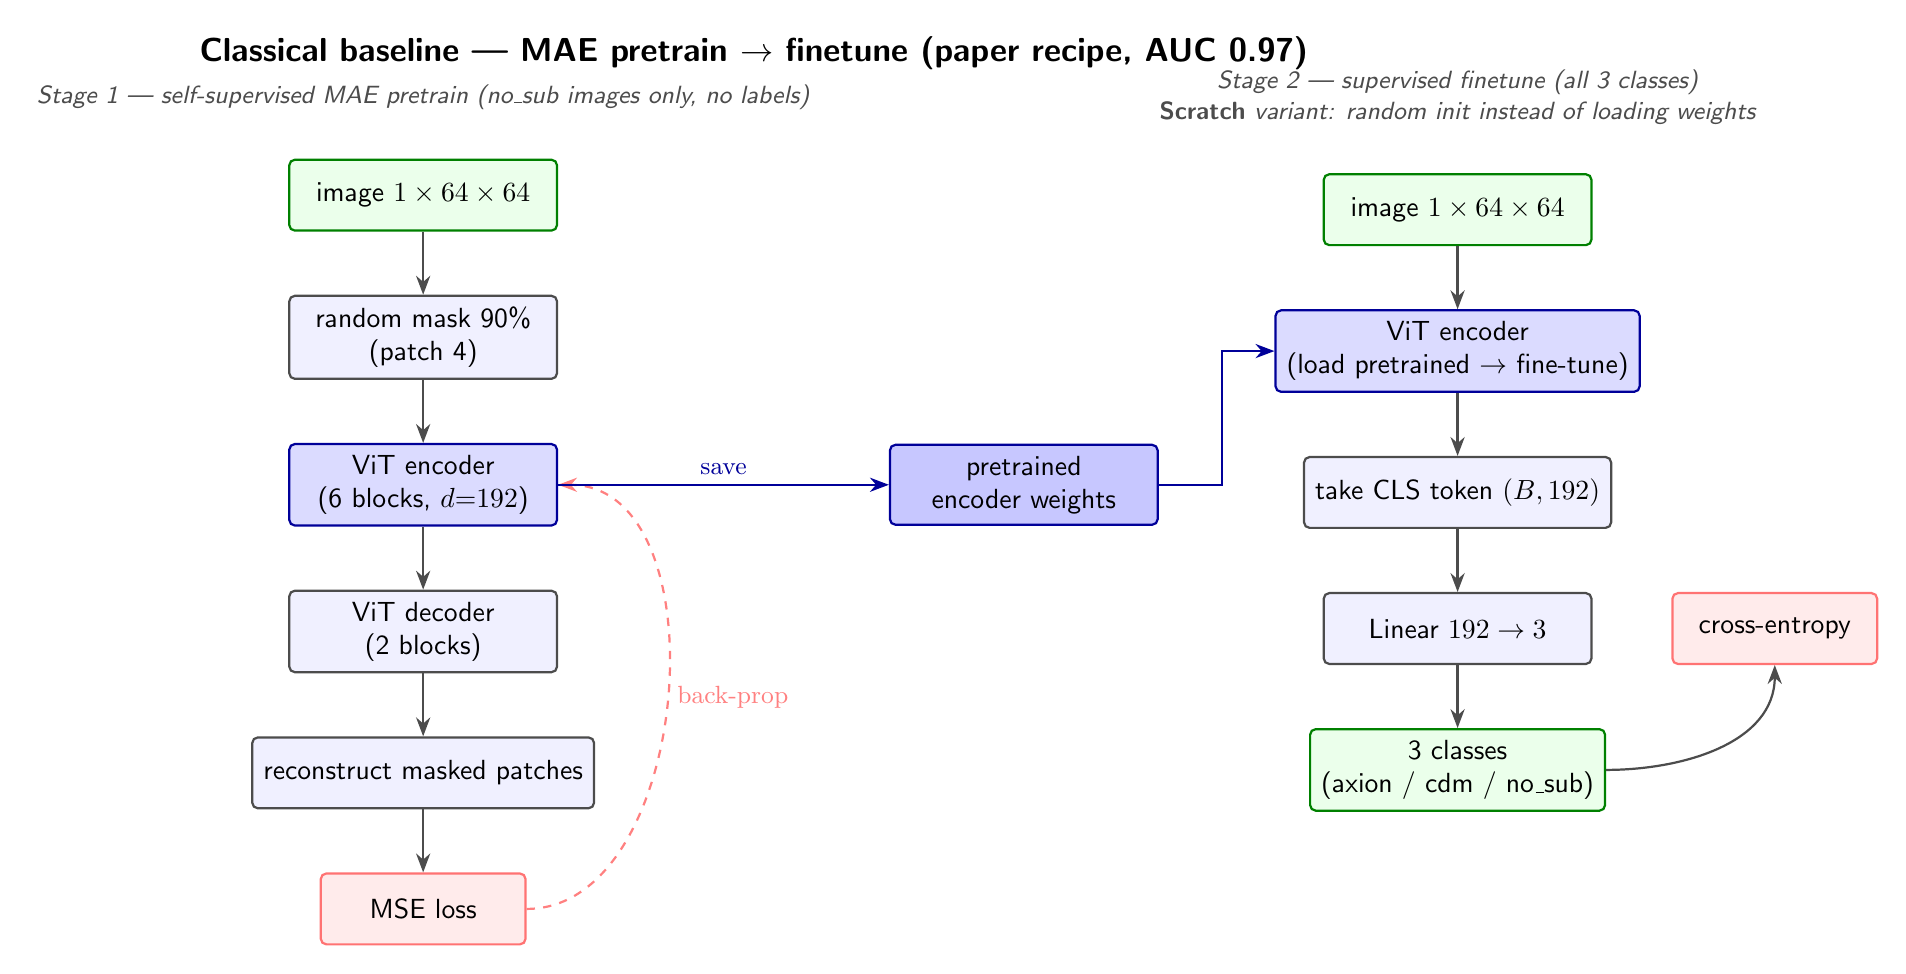
\begin{tikzpicture}[
  font=\sffamily,
  node distance=8mm,
  box/.style={rectangle,rounded corners=2pt,draw=black!70,thick,fill=blue!6,
              minimum height=9mm,minimum width=34mm,align=center,inner sep=4pt},
  io/.style={box,fill=green!8,draw=green!50!black},
  loss/.style={box,fill=red!8,draw=red!55,minimum width=26mm},
  enc/.style={box,fill=blue!14,draw=blue!60!black},
  arr/.style={-{Stealth[length=2.4mm]},thick,black!70},
  lbl/.style={font=\sffamily\small\itshape,gray!60!black},
]
% ===== Stage 1: self-supervised MAE pretrain =====
\node[lbl] (s1) {Stage 1 — self-supervised MAE pretrain (no\_sub images only, no labels)};
\node[io,below=5mm of s1] (img1) {image $1\times64\times64$};
\node[box,below=of img1] (mask) {random mask 90\%\\(patch 4)};
\node[enc,below=of mask] (enc1) {ViT encoder\\(6 blocks, $d{=}192$)};
\node[box,below=of enc1] (dec) {ViT decoder\\(2 blocks)};
\node[box,below=of dec] (rec) {reconstruct masked patches};
\node[loss,below=of rec] (mse) {MSE loss};
\draw[arr](img1)--(mask); \draw[arr](mask)--(enc1); \draw[arr](enc1)--(dec);
\draw[arr](dec)--(rec); \draw[arr](rec)--(mse);
\draw[arr,dashed,red!50] (mse.east) to[out=0,in=0] node[right,font=\small]{back-prop} (enc1.east);

% encoder weights handoff
\node[enc,right=42mm of enc1,fill=blue!22] (encW) {pretrained\\encoder weights};
\draw[arr,blue!60!black,thick] (enc1.east) -- node[above,font=\small]{save} (encW.west);

% ===== Stage 2: supervised finetune =====
\node[lbl,right=42mm of s1,align=center] (s2) {Stage 2 — supervised finetune (all 3 classes)\\\textbf{Scratch} variant: random init instead of loading weights};
\node[io,below=5mm of s2] (img2) {image $1\times64\times64$};
\node[enc,below=of img2] (enc2) {ViT encoder\\(load pretrained $\rightarrow$ fine-tune)};
\node[box,below=of enc2] (cls) {take CLS token $(B,192)$};
\node[box,below=of cls] (head) {Linear $192\rightarrow3$};
\node[io,below=of head] (out) {3 classes\\(axion / cdm / no\_sub)};
\node[loss,right=10mm of head] (ce) {cross-entropy};
\draw[arr](img2)--(enc2); \draw[arr](enc2)--(cls); \draw[arr](cls)--(head);
\draw[arr](head)--(out); \draw[arr](out.east) to[out=0,in=-90] (ce.south);
\draw[arr,blue!60!black,thick] (encW.east) -- ($(encW.east)+(0.8,0)$) |- (enc2.west);

\node[font=\sffamily\large\bfseries,above=10mm of img1,xshift=42mm]
  {Classical baseline — MAE pretrain $\rightarrow$ finetune (paper recipe, AUC 0.97)};
\end{tikzpicture}
\end{document}
